\documentclass{cmc}
\usepackage{makecell}
\begin{document}

\pagestyle{fancy}
\lhead{\textit{\textbf{Computational Motor Control, Spring 2019} \\
    Webots exercise, Lab 9, GRADED}} \rhead{Student \\ Names}

\section*{Student names: \ldots (please update)}

\textit{Instructions: Update this file (or recreate a similar one, e.g.\ in
  Word) to prepare your answers to the questions. Feel free to add text,
  equations and figures as needed. Hand-written notes, e.g.\ for the development
  of equations, can also be included e.g.\ as pictures (from your cell phone or
  from a scanner).  \textbf{\corr{This lab is graded.}} and needs to be
  submitted before the \textbf{\corr{Deadline : Wednesday 15-05-2019
      Midnight. You only need to submit one final report for all of the
      following exercises combined henceforth.}} Please submit both the source
  file (*.doc/*.tex) and a pdf of your document, as well as all the used and
  updated Python functions in a single zipped file called
  \corr{final\_report\_name1\_name2\_name3.zip} where name\# are the team
  member’s last names.  \corr{Please submit only one report per team!}}
\\

\corr{\textit{NOTE : }}The following exercises on Salamandra robotica are based
on the research of \cite{Crespi2013}, \cite{Karakasiliotis2013} and
\cite{ijspeert2007swimming}.

\section*{Swimming with Salamandra robotica – CPG Model}
\label{sec:exploring-swimming}

In this exercise you will control a salamander-like robot Salamandra
robotica for which you will use Python and the dynamics simulator
Webots. Now you have an opportunity to use what you’ve learned until
now to make the robot swim (and eventually walk). In order to do this,
you should implement a CPG based swimming controller, similarly to the
architecture shown in Figure~\ref{fig:controller-model}.

In the folder Webots you will find sub folders containing the simulated
world file and Python codes describing the controller.
\corr{\textbf{\textit{NOTE : }}Do not change the relative positions of
  files within those folders.}

\begin{figure}[h]
  \centering
  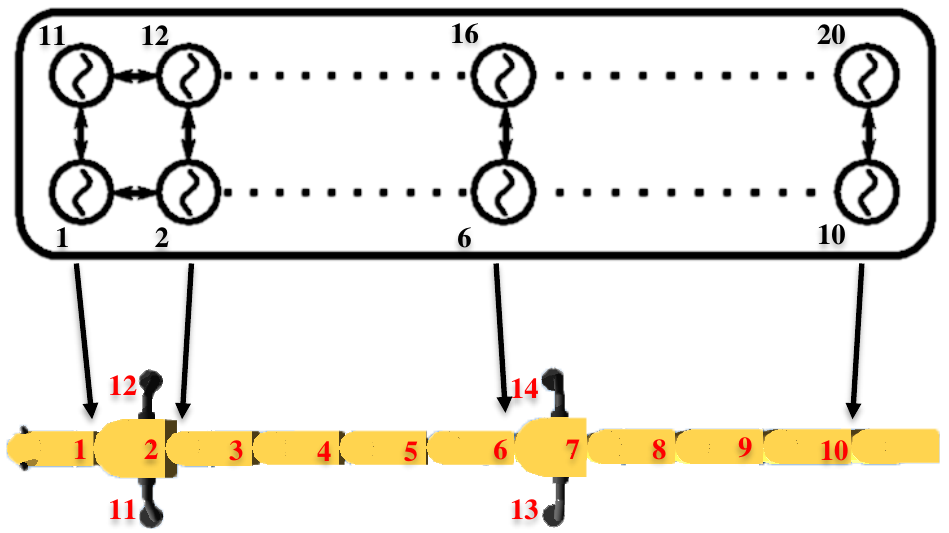
\includegraphics[width=0.5\textwidth]{figures/model_controller.png}
  \caption[Controller model]{A double chain of oscillators controlling
    the robot’s spine.}
  \label{fig:controller-model}
\end{figure}

\begin{figure}[ht]
  \centering 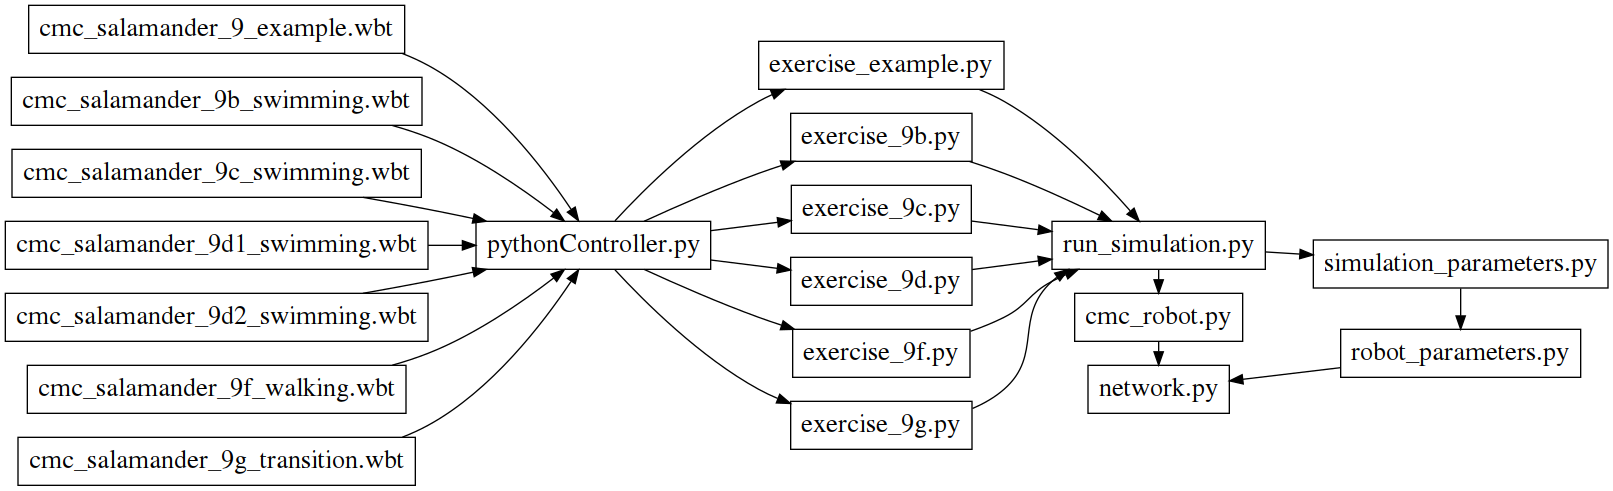
\includegraphics[width=1.0\textwidth]{figures/files}
  \caption{\label{fig:files} Exercise files dependencies. In this lab, you will
    be modifying \fileref{exercise1.py} and \fileref{pendulum\_system.py}}
\end{figure}

% \newpage

\subsection*{Code organization}
\label{subsec:code}

\begin{itemize}
\item \corr{\textbf{Webots::worlds::cmc\_salamander\_\#.wbt}} - These are the
  world files which describe the worlds and allow to run the simulations. You
  can run a simulation by running this file with Webots. It also automatically
  loads the pythonController. Note that each of these files will also run the
  appropriate \corr{exercise\_\#.py} such that you can run each exercise
  separately. Note that the simulation of the exercises may close immediately as
  they are not implemented yet. Only \corr{cmc\_salamander\_9\_example.wbt} will
  run for a few seconds before closing.
\item \corr{\textbf{Webots::controllers::pythonController::exercise\_\#.py}} -
  To be used to implement and answer the respective exercise questions. Note
  that \corr{exercise\_example.py} is provided as an example to show how to run
  a parameter sweep. Note that network parameters can be provided here.
\item \corr{\textbf{Webots::controllers::pythonController::pythonController.py}}
  - The main robot controller is implemented in pythonController.py. This file
  is the main file called by Webots during simulations and can call classes and
  functions from other files to control the robot and log data. This file is
  mainly used for calling the appropriate \corr{exercise\_\#.py} file. Note that
  by default the simulation will close Webots when it finishes. If you do not
  want Webots to close, you can comment the following line:
  \texttt{world.simulationQuit(0)}.
\item \corr{\textbf{Webots::controllers::pythonController::run\_simulations.py}}
  There is a run\_simulation.py function which is provided for convenience
  to easily run multiple simulations with different parameters. You are free to
  implement other functions to run simulations as necessary.
\item \corr{\textbf{Webots::controllers::pythonController::cmc\_robot.py}} -
  Contains the SalamanderCMC class, which is used for controlling and logging
  the robot.
\item
  \corr{\textbf{Webots::controllers::pythonController::experiment\_logger.py}} -
  Contains the codes for logging the simulation. Feel free to modify this file
  to extend the logging capabilities. Note that the logging makes use of
  Numpy.savez to save the data.
\item \corr{\textbf{Webots::controllers::pythonController::network.py}} - This
  file contains the different classes and functions for the CPG network and the
  Ordinary Differential Equations (ODEs). You can implement the network
  parameters and the ODEs here. Note that some parameters can be obtained from
  pythonController.py to help you control the values.
\item
  \corr{\textbf{Webots::controllers::pythonController::robot\_parameters.py}} -
  This file contains the different classes and functions for the parameters of
  the robot, including the CPG network parameters. You can implement the network
  parameters here. Note that some parameters can be obtained from
  SimulationParameters class in \corr{simulation\_parameters.py} and sent by
  \corr{exercise\_\#.py} to help you control the values (refer to example).
\item
  \corr{\textbf{Webots::controllers::pythonController::simulation\_parameters.py}}
  - This file contains the SimulationParameters class and is provided for
  convenience to send parameters to the setup of the network parameters in
  \corr{robot\_parameters.py}. All the values provided in SimulationParameters
  are actually logged in \corr{cmc\_robot.py}, so you can also reload these
  parameters when analyzing the results of a simulation.
\item \corr{\textbf{Webots::controllers::pythonController::solvers.py}} - This
  features fixed time-step solvers which will can are used by network.py for
  solving the ODE at each time-step. Feel free to switch between the Euler and
  the Runge-Kutta methods. \textit{You do not need to modify this files.}
\item \corr{\textbf{Webots::controllers::pythonController::run\_network.py}} -
  By running the script from Python, Webots will be bypassed and you will run
  the network without a physics simulation. Make sure to use this file for
  question 9a to help you with setting up the CPG network equations and
  parameters and to analyze its behavior. This is useful for debugging purposes
  and rapid controller development since starting the Webots simulation with
  physics takes more time.
\item \corr{\textbf{Webots::controllers::pythonController::plot\_results.py}} -
  Use this file to load and plot the results from the simulation. This code runs
  with the original pythonController provided.
\item \corr{\textbf{Webots::controllers::pythonController::parse\_args.py}} -
  Used to parse command line arguments for run\_network.py and plot\_results.py
  and determine if plots should be shown or saved directly. \textit{You do not
    need to modify this files.}
\item \corr{\textbf{Webots::controllers::pythonController::save\_figures.py}} -
  Contains the functions to automatically detect and save figures. \textit{You
    do not need to modify this files.}
\item
  \corr{\textbf{Webots::controllers::pythonController::exercise\_example.py}} -
  Contains the example code structure to help you familiarize with the other
  exercises. \textit{You do not need to modify this files.}
\end{itemize}

% \newpage

\section*{Prerequisites}

\subsection*{Make sure you have successfully installed Webots by
  following the instructions outlined in Lab 7}

\subsection*{Complete the tutorial and practice examples of Webots as
  outlined in Lab 7}

\subsection*{Open the \fileref{Webots::worlds::cmc\_salamander\_9\_example.wbt} file
  in Webots. This should launch the Salamandra robotica model in
  simulation world}

\subsection*{Running the simulation}
Now when you run the simulation, the Salamandra robotica model should
float on the water with no errors in the Webots console dialog. At
this point you can now start to work on implementing your exercises.

\newpage

\section*{Questions}

The exercises are organized such that you will have to first implement the
oscillator network model in \corr{run\_network.py} code and analyze it before
connecting it to the body in the Webots world.  Exercise 9a describes the
questions needed to implement the oscillator models. After completing exercise
9a you should have an oscillator network including both the spinal CPG and limb
CPG.

Using the network implemented in exercise 9a you can explore the swimming,
walking and transition behaviors in the Salamandra robotica model using Webots
and complete the exercises 9b to 9g.

\subsection*{9a. Implement a double chain of oscillators along with
  limb CPG's}
\label{sec:implement-chain}

Salamandra robotica has 10 joints along its spine and 1 joint for each
limb. The controller

\begin{equation}
  \label{eq:dphase}
  \dot{\theta}_i = 2 \pi f + \sum_j r_j w_{ij} sin(\theta_j - \theta_i - \phi_{ij})
\end{equation}

\begin{equation}
  \label{eq:dr}
  \dot{r}_i = a (R_i - r_i)
\end{equation}

\begin{equation}
  \label{eq:output}
  q_i = r_i(1 + cos(\theta_i)) - r_{i+10}(1 + cos(\theta_{i+10})) \text{ if body joint}
\end{equation}

with $ \theta_i $ the oscillator phase, f the frequency, $ w{_ij} $ the coupling
weights, $ \phi_{ij} $ the nominal phase lag (phase bias), $ r_i $ the
oscillator amplitude, $ R_i $ the nominal amplitude, $ a $ the convergence
factor and $ q_i $ the spinal joint angles.


\begin{enumerate}
\item Implement the double chain oscillator model using the functions
  \fileref{network.py::network\_ode}. Test your implementation by running the
  network using \fileref{run\_network.py}. For the network parameters check
  lecture slides (pay attention to different number of segments). You can also
  find more information in \cite{ijspeert2007swimming} (especially in the
  supplementary material). You can set all the network parameters in the
  \fileref{robot\_parameters.py::RobotParameters}. To facilitate your work, you
  could start by only implementing the network for the body oscillators
  ($i=[0, ..., 19]$) and ignoring the leg oscillators ($i=[20, ..., 23]$). Refer
  to \corr{network::RobotState} and
  \corr{robot\_parameters.py::}\-\corr{RobotParameters} for the dimensions of
  the state and the network parameters respectively.

\item Implement the output of your CPG network to generate the spinal joint
  angles according to equation \ref{eq:output}. Implement this in the function
  \fileref{network.py::motor\_output}. Verify your implementation in by running
  the Python file \fileref{run\_network.py}.  Use the functions in
  \fileref{plot\_results.py} to report your spinal joint angles $q_i$.

\item Implement a drive and show that your network can generate swimming and
  walking patterns similarly to \cite{ijspeert2007swimming}.


  \textbf{Hint:} The state for the network ODE is of size 48 where the first 24
  elements correspond to the oscillator phases $\theta_i$ of the oscillators and
  the last 24 elements correspond to the amplitude $r_i$. The initial state is
  set in the init of \corr{network.py::SalamanderNetwork}.
\end{enumerate}


\subsection*{9b. Effects of amplitude and phase lags on swimming
  performance}
\label{sec:amplitude-phase-performance}

Now that you have implemented the controller, it is time to run experiments to
study its behaviour. How does phase lag and oscillation amplitude influence the
speed and energy? Use the provided \corr{run\_simulation.py::run\_simulation()}
to run a grid search to explore the robot behavior for different combinations of
amplitudes and phase lags. Use \corr{plot\_results.py} to load and plot the
logged data from the simulation. Feel free to extend the logging in
\corr{cmc\_robot.py} to show additional measurements if necessary. Include 2D/3D
plots showing your grid search results and discuss them. How do your findings
compare to the wavelengths observed in the salamander?

% Run the grid search twice, for frequencies of 1Hz and 2Hz.

\begin{itemize}
\item \textbf{Hint 1:} To use the grid search, check out the function
  \corr{run\_simulation.py::run\_simulation()} and the example provided in
  \corr{exercise\_example.py}. This function takes the desired parameters as a
  list of SimulationParameters objects (found in
  \corr{simulation\_parameters.py}) and runs the simulation. Note that the
  results are logged as simulation\_\#.npz in a specified log folder. After the
  grid search finishes, the simulation will close, you can remove this feature
  by commenting world.simulationQuit(0) in \corr{pythonController.py::main()}.
\item \textbf{Hint 2:} An example how to load and visualise grid
  search results is already implemented in
  \corr{plot\_results.py::main()}. Pay attention to the name of the
  folder and the log files you are loading. Before starting a new grid
  search, change the name of the logs destination folder where the
  results will be stored. In case a grid search failed, it may be
  safer to delete the previous logs to avoid influencing new results
  by mistake.
\item \textbf{Hint 3:} Estimate how long it will take to finish the
  grid search. Our suggestion is to choose wisely lower and upper
  limits of parameter vectors and choose a reasonable number of
  samples. To speed-up a simulation, make sure to run Webots in a fast
  mode.
\item \textbf{Hint 4:} Energy can be estimated by integrating the
  product of instantaneous joint velocities and torques. Feel free to
  propose your own energy metrics, just make sure to include the
  justification.
\end{itemize}


\subsection*{9c. Amplitude gradient}
\label{sec:amplitude-gradient}

\begin{enumerate}
\item So far we considered constant undulation amplitudes along the body for
  swimming. Implement a linear distribution of amplitudes along the spine,
  parametrized with two parameters: amplitudes of the first (Rhead) and last
  (Rtail) oscillator in the spine (corresponding to the first and last
  motor). To do so, you can add a parameter amplitudes=[Rhead, Rtail] in
  \corr{simulation\_parameters.py::SimulationParameters}. Don't forget to modify
  \corr{robot\_parameters.py::}\-\corr{RobotParameters::set\_nominal\_amplitudes()}
  and interpolate the amplitude gradient between values Rhead and Rtail within
  the function. Note that you can then provide this amplitudes parameter from
  \corr{exercise\_9b.py}.
\item Run a grid search over different values of parameters Rhead and
  Rtail (use the same range for both parameters). How does the
  amplitude gradient influence swimming performance (speed, energy)?
  Include 3D plots showing your grid search results. Do it once, for
  frequency 1Hz and total phase lag of $2\pi$ along the spine.
\item How is the salamander moving (with respect to different body
  amplitudes)?  How do your findings in 2) compare to body
  deformations in the salamander?  Based on your explorations, what
  could be possible explanations why the salamander moves the way it
  does?
\end{enumerate}


\subsection*{9d. Turning and backwards swimming}
\label{sec:turning-backwards}

\begin{enumerate}
\item How do you need to modulate the CPG network (\corr{network.py})
  in order to induce turning?  Implement this in the Webots model and
  plot example GPS trajectories and spine angles.
\item How could you let the robot swim backwards? Explain and plot
  example GPS trajectories and spine angles.
\end{enumerate}



\subsection*{9e. Cancelled}

\subsection*{9f. Limb – Spine coordination}
\label{sec:limb-spine-coordination}

In this next part you will explore the importance of a proper coordination
between the spine and the limb movement for walking.

\begin{enumerate}
\item Change the drive to a value used for walking and verify that the robot
  walks
\item Analyze the spine movement: What are your phase lags along the spine
  during walking? How does the spine movement compare to the one used for
  swimming?
\item Notice that the phase between limb and spine oscillators affects the
  robot’s walking speed. Run a parameter search on the phase offset between
  limbs and spine. Set the nominal radius R to 0.3 [rad]. Include plots showing
  how the phase offset influences walking speed and comment the results. How do
  your findings compare to body deformations in the salamander while walking?
\item Explore the influence of the oscillation amplitude along the body with
  respect to the walking speed of the robot. Run a parameter search on the
  nominal radius R with a fixed phase offset between limbs and the spine. For
  the phase offset take the optimal value from the previous sub-exercise. While
  exploring R, start from 0 (no body bending).
\end{enumerate}

Include plots showing how the oscillation radius influences walking speed and
comment on the results.



\subsection*{9g. Land-to-water transitions}

\begin{enumerate}
\item In this exercise you will explore the gait switching mechanism. The gait
  switching is generated by a high level drive signal which interacts with the
  saturation functions that you should have implemented in 9a. Implement a new
  experiment which uses the x-coordinate of the robot in the world retrieved
  from a GPS reading (See \texttt{self.gps.getValues()} in
  \corr{cmc\_robot::log\_iteration()} for an example). Based on the GPS reading,
  you should determine if the robot should walk (it’s on land) or swim (it
  reached water). Depending on the current position of the robot, you should
  modify the drive such that it switches gait appropriately.
\item Run the Webots simulation and report spine and limb angles, together with
  the x coordinate from the GPS signal. Record a video showing the transition
  from land to water and submit the video together with this report.
\item (BONUS) Achieve water-to-land transition. Report spine and limb angles,
  the x-coordinate of the GPS and record a video.
\end{enumerate}


\textbf{Hint:} Use Webots’ internal video recording tool to easily record
videos.



\newpage

\bibliography{lab9}
\label{sec:references}
\bibliographystyle{ieeetr}


% \newpage

% \section*{APPENDIX}
% \label{sec:appendix}

\end{document}

%%% Local Variables:
%%% mode: latex
%%% TeX-master: t
%%% End: